\documentclass[conference]{IEEEtran}

% This is the setup file. It contains usepackage commands, acronyms, and other
% useful commands needed to set up the paper. Uncomment the relevant sections to
% use them.

% Packages. Make sure your LaTeX distribution actually has the packages!
\usepackage{acro}  % Acronyms
\usepackage{amsmath} % cases environment
\usepackage{color}  % Used to highlight comments
\usepackage{graphicx}  % To allow figures
\usepackage{msc}  % Message sequence charts
\usepackage{paralist}  % For tighter lists
\usepackage{xspace}  % For spacing after user-defined commands and others.
\usepackage[hyphens]{url}  % To make URLs display correctly in citations. The
                           % hyphens option allows line breaks after hyphens.
\usepackage{hyperref}  % Hyperlinks in citations and references


% Acronym definitions (requires acro package)

\DeclareAcronym{ca}{
  short={CA},
  long={certificate authority},
  long-plural-form={certificate authorities},
  alt={certification authority},
}
\DeclareAcronym{crl}{
  short={CRL},
  long={certificate revocation list},
}
\DeclareAcronym{ct}{
  short={CT},
  long={Certificate Transparency},
}
\DeclareAcronym{hsts}{
  short={HSTS},
  long={HTTP Strict Transport Security},
  short-indefinite={an},
  long-indefinite={an},
}
\DeclareAcronym{https}{
  short={HTTPS},
  long={HTTP over TLS},
  short-indefinite={an},
  long-indefinite={an},
}
\DeclareAcronym{mitm}{
  short={MITM},
  long={man-in-the-middle},
  short-indefinite={an},
}
\DeclareAcronym{mmd}{
  short={MMD},
  long={maximum merge delay},
  short-indefinite={an},
}
\DeclareAcronym{name}{
  short={CTAPS},
  long={Certificate Transparency with Automated Policies and Signaling},
}
\DeclareAcronym{oid}{
  short={OID},
  long={object identifier},
  short-indefinite={an},
  long-indefinite={an},
}
\DeclareAcronym{pki}{
  short={PKI},
  long={public-key infrastructure},
}
\DeclareAcronym{sct}{
  short={SCT},
  long={signed certificate timestamp},
  short-indefinite={an},
}
\DeclareAcronym{sth}{
  short={STH},
  long={signed tree head},
  short-indefinite={an},
}
\DeclareAcronym{tls}{
  short={TLS},
  long={Transport Layer Security},
}
\DeclareAcronym{x509}{
  short={X.509},
  long={X.509 Version 3},
  short-indefinite={an},
  long-indefinite={an},
}

% Example acronym definition. Uncomment to use.
%\DeclareAcronym{pki}{
  %short={PKI},
  %long={public-key infrastructure},
  %%short-plural={s},  % default
  %%long-plural={s},  % default
  %%long-plural-form={},  % use for irregular plurals
  %%short-indefinite={a},  % plural
  %%long-indefinite={a},  %plural
  %%alt={},  % alternate form
  %%alt-indefinite={a},
  %%short-format={},  % formatting for first short use
  %%long-format={},  % formatting for first long use
  %%first-long-format={\capitalisewords},  % must use mfirstuc package
  %%pdfstring={},  % string to use with hyperref section headings, etc.
%}



% User-defined commands go here.

\newcommand{\steve}[1]{\textcolor{magenta}{[SM: #1]}}
\newcommand{\draft}[1]{\textcolor{blue}{[Draft text: #1]}}
\newcommand{\emxs}[1]{\ensuremath{#1}\xspace}

\newcommand{\evidence}{\emxs{E}}
\newcommand{\hashfunc}{\emxs{H}}
\newcommand{\nodehash}{\emxs{h}}
\newcommand{\regstr}{\emxs{S}}

%\newcommand\definitionautorefname{Definition}
\renewcommand*{\equationautorefname}{Equation}
\renewcommand*{\figureautorefname}{Figure}
\renewcommand*{\sectionautorefname}{Section}
%\renewcommand*{\itemautorefname}{Definition}
\let\subsectionautorefname\sectionautorefname
%\newcommand{\algorithmautorefname}{Algorithm}



\setmsckeyword{}


% Fix ugly citation style: [1],[2] --> [1,2]

%\usepackage[noadjust]{cite}
%\renewcommand{\citepunct}{, }
%\renewcommand{\citedash}{--}

% Compression tricks - use if we need more space.

%\geometry{tmargin=.7in,bmargin=.7in,lmargin=.7in,rmargin=.7in}
%\renewcommand{\baselinestretch}{0.99}

% Aggressive space hacks. Use only in case of emergency!
%\usepackage[font=footnotesize]{caption}
%\usepackage{titlesec}
%\titlespacing\section{0pt}{5pt plus 1pt minus 0pt}{1pt minus 1pt}
%\titlespacing\subsection{0pt}{4pt plus 2pt minus 0pt}{1pt minus 0pt}
%\titleformat{name=\section}{\fontsize{11.7pt}{14pt}\bfseries}{\thesection}{1em}{}
%\titleformat{name=\subsection}{\fontsize{10.73pt}{12.87pt}\bfseries}{\thesubsection}{1em}{}
%\usepackage[final,babel,step=1,stretch=30,shrink=40]{microtype}
%\usepackage[all=normal,lists,paragraphs,wordspacing,leading]{savetrees}


\begin{document}

\title{
  Title
}
\author{
  Authors
}

%\author{\IEEEauthorblockN{Michael Shell}
%\IEEEauthorblockA{Georgia Institute of Technology\\
%someemail@somedomain.com}
%\and
%\IEEEauthorblockN{Homer Simpson}
%\IEEEauthorblockA{Twentieth Century Fox\\
%homer@thesimpsons.com}
%\and
%\IEEEauthorblockN{James Kirk\\ and Montgomery Scott}
%\IEEEauthorblockA{Starfleet Academy\\
%someemail@somedomain.com}}

\maketitle

%\begingroup
%\let\thefootnote\relax\footnotetext{This paper is an extended version of any
%conference or journal publication of this work, and is intended for internal
%use. As such, it contains many details not necessary to understand the core idea
%of the work.}
%\endgroup

\begin{abstract}
  \steve{TODO}

\end{abstract}

\section{Introduction}
\label{sec:intro}

%Some questions to think about:
%\begin{compactitem}
%\item How can we move toward a world in which domains use multiple independent
  %certificate chains?
%\item How do we validate a self-signed certificate?
%\item What does it mean to have trust agility?
%\item Does the use of multiple independent certificate chains provide better
  %security and agility?
%\end{compactitem}

\acs{https}, built on \ac{tls}~\cite{rfc5246} and the Web \ac{pki}, lies at the
heart of secure end-to-end communication on the Web. \Acp{ca}, who vouch for the
binding between a domain's name and its public key, play a critical role in the
Web \ac{pki}. \Iac{ca}'s failure to correctly sign this binding in the form of a
public key certificate can lead to \iac{mitm} attack, allowing an adversary to
intercept and modify all communication between a client and domain. Recent years
have seen a plethora of these failures, both
accidental~\cite{sleevi2015sustaining} and
intentional~\cite{valsorda2015komodia}.

The failures of \acp{ca} continually remind us of the weakest-link security of
the Web \ac{pki}: a single misbehaving \ac{ca} can expose a domain to \ac{mitm}
attacks. Because we cannot prevent \acp{ca} from misissuing certificates,
protecting clients from these \ac{mitm} attacks entails making the \ac{pki}
resilient to certificate misissuance by enabling clients to detect and reject
misissued certificates. However, only domains themselves can with certainty
identify certificates misissued in their name. Clients therefore need a way to
determine a domain's \emph{certificate policy} (i.e., criteria for which
certificates the clients should consider correctly issued).

So far, proposed systems for communicating policy information to clients have
not gained traction in practice. These systems introduce additional trusted
parties~\cite{kim2013accountable} or assume that the entire Web will increase
its security at once~\cite{basin2014arpki}. These shortcomings motivate the
problem of designing a simple and deployable policy mechanism that requires
minimal effort from domains. \steve{The last part isn't motivated well; it would
  be nice if we could show that most policies are overkill for preventing
\ac{mitm} attacks that could have resulted from recent \ac{ca} failures.}

%The Web's \ac{pki} enables client browsers to authenticate the public keys of
%the domains they communicate with, and together with the \ac{tls}
%protocol~\cite{rfc5246} allows a client and domain to establish an end-to-end
%secure communication channel through \acs{https}. In the Web \ac{pki},
%trusted third parties called \emph{\acp{ca}} vouch for the binding between a
%domain's name and its public key. The correct operation of \acp{ca} are critical
%to the security of the Web \ac{pki}, and failures can lead to the client
%establishing a secure channel with the wrong domain. In some cases this
%scenario can lead to a \emph{\ac{mitm} attack}, in which even though the
%confidentiality and integrity guarantees of communication over \ac{tls} hold,
%they provide no benefit because an adversary is impersonating the client and
%domain to each other and can read and modify all communication between them.

%While there are many proposals (enumerated in \autoref{sec:related}) to fix the
%Web \ac{pki} by deterring, preventing, or recovering from \ac{ca} misbehavior,
%Google's \emph{\ac{ct}} system~\cite{rfc6962} has recently emerged as a widely
%deployed example of such a system, being scheduled for full deployment in
%October 2017. \ac{ct} does not prevent \ac{mitm} attacks, but rather enables
%widespread detection of \ac{ca} misbehavior. In \ac{ct}, a set of \emph{public
%logs} maintain a database of certificates they have observed (primarily sent to
%them by the \acp{ca} themselves) and provide cryptographic proofs called
%\emph{\acp{sct}} that show when these certificates were submitted to the log.
%Clients do not accept certificates unless they are sent with a requisite number
%of these \acp{sct}, ensuring that an adversary cannot use an unauthorized
%certificate for \ac{mitm} attacks without first exposing that certificate to the
%world.

%However, \ac{ct} has several notable shortcomings. \ac{ct} does not make
%\ac{mitm} attack prevention an explicit goal, but specifies the behavior of
%\emph{monitors}, who periodically download newly logged certificates and check
%for suspicious certificates. However, only domains know which certificates they
%have authorized, and \ac{ct} does not allow domains to check logs for
%certificates issued in their name. This disparity means that some manual effort,
%on the part of the monitors, domains, or both, is required to prevent \ac{mitm}
%attacks that result from unauthorized certificates. Both monitors and domains
%face hurdles due to this manual effort.

%With the increasing deployment of \ac{https} through certificate services such
%as Let's Encrypt,\footnote{\texttt{https://letsencrypt.org/}} monitors may not
%be able to keep up with the number of suspicious certificates that require
%further manual investigation. Previous work enables domains to alleviate this
%pressure on monitors by explicitly supplying \emph{policies} that specify
%criteria that a domain's certificates should meet, but it is not clear that the
%expressiveness of these policies and the burden they impose on domain operators
%is worth the benefit of protecting them from common certificate misissuances. We
%therefore seek a simpler, more automated system for specifying certificate
%policies through the \ac{ct} infrastructure. In particular, we aim to move
%towards \iac{pki} in which one-off mistakes by \acp{ca} do not expose domains to
%\ac{mitm} attacks.

Unfortunately, even with such policies, we still fall short of a truly secure
\ac{pki}. Domains may not only have different policies, but some domains may not
have policies at all because they do not deploy \ac{https}. Because we
realistically expect a world of partial deployment in which the set of deploying
domains increases incrementally over time, we need a mechanism to inform clients
\emph{when} to expect a certificate policy, not just \emph{what} policy to
expect. Moreover, this mechanism must be external to the Web \ac{pki} because it
indicates certification in the Web \ac{pki} itself. We call the problem of
designing such a mechanism the \emph{signaling} problem.

%These policies only exist for domains that actually deploy \ac{https};
%therefore, an adversary can bypass these protections by convincing the client
%that the target domain does not deploy \ac{https} at all (e.g., by blocking
%connections to port 443 over which domains usually serve \ac{https}). We
%therefore need a \emph{signaling} mechanism that securely indicates whether or
%not the client should expect the domain to deploy \ac{https}. Some existing
%approaches are opt-in, meaning that domains must explicitly register for these
%mechanisms, and thus only provide signaling for some sites (e.g., popular
%sites). Furthermore, the opt-in process is prone to misconfigurations, such as
%domains accidentally signaling that a subdomain deploys \ac{https}, thus
%rendering that part of the site inaccessible to clients. Other approaches
%require clients to perform online checks, degrading connection latency. Is it
%possible to improve on these approaches by reducing the action required by
%domains and by broadening the scope of domains that can signal \ac{https}
%deployment \emph{without} significantly increasing connection latency?

Existing approaches to the signaling problem
(\autoref{sec:background:signaling}) suffer from critical shortcomings. Some
require domains to opt in using a process prone to misconfiguration, and render
the domain inaccessible if misconfiguration occurs. Approaches that store
deployment information locally only signal \ac{https} deployment in a subset of
sites due to storage costs, and approaches that rely on external information
incur significant latency penalties and introduce additional trusted parties. We
therefore observe the need to address the signaling problem with a solution that
allows clients to confidently distinguish a site that deploys \ac{https} without
imposing performance penalties or trust assumptions.

To address the problems of managing certificate policies and of signaling
\ac{https} deployment in a simple and practical manner, we propose \ac{name}, a
system that \steve{gradually} increases the resilience of the Web \ac{pki}
against misbehaving \acp{ca}. \ac{name} leverages Google's
\ac{ct}~\cite{rfc6698} infrastructure, which relies on \emph{public logs} that
maintain a database of all issued certificates in the Web \ac{pki}.
%Because all certificates must be publicly logged to be accepted in Chrome
%browsers starting in October
%2017,\footnote{\url{https://cabforum.org/2016/10/19/2016-10-19-20-f2f-meeting-39-minutes/}}
\ac{name} repurposes these logs to also maintain certificate policies. \ac{name}
also achieves simplicity of policies by only tracking the number of \ac{ca}
certificates for a given key a client should expect. This simple approach also
means that for the vast majority of cases, domains do not need to change they
way they obtain certificates, and in fact only requires domains to occasionally
fetch information from a public log.

\ac{name} uses data from \ac{ct} logs and from Censys~\cite{durumeric2015search}
scans of \ac{https} sites to provide a complete view of all sites deploying
\ac{https}. Using data from these sources also means that domains do not have to
opt in to signal \ac{https} deployment. By using finite state methods and data
compression techniques, \ac{name} can also succinctly encode the set of sites
deploying \ac{https} to achieve fast, local signaling with efficient updates and
minimal additional connection latency.

In summary, this paper makes the following contributions:
\begin{compactitem}
\item It leverages \ac{ct} to propose a simple, deployable, and automated
  mechanism for maintaining and disseminating domain certificate policies.
\item It leverages finite state automata and data compression to present  a
  succinct design for communicating the set of sites deploying \ac{https}.
\item It shows through a comparative evaluation that \ac{name} requires only
  \steve{} extra communication, \steve{} additional storage, and \steve{}
  additional latency.
\end{compactitem}

%The Web \ac{pki} has seen several important improvements in recent years.
%\steve{Summary of CT, CAA, DANE, CAge, CRLite}

%Because \acp{ca} are trusted parties in the \ac{tls} \ac{pki}, they can enable
%\ac{mitm} attacks if they misbehave. Unfortunately, they have done so multiple
%times over the years, due to social engineering
%attacks~\cite{microsoft2001erroneous}, network breaches~\cite{comodo2011fraud,
  %hoogstraaten2012black}, operational errors~\cite{zusman2009sub,
  %langley2013enhancing, somogyi2015improved, sleevi2015sustaining}, or malicious
  %intent~\cite{percoco2012clarifying, langley2013further,
  %langley2015maintaining}. While in many cases the rogue certificates were
  %quickly detected and revoked, in some cases the certificates were actually
  %used in the wild in \ac{mitm} attacks~\cite{nightingale2011diginotar}. These
  %attacks are particularly noxious because the victim website may never find out
  %that it is being impersonated. Indeed, we have seen instances of targeted
  %attacks using fake certificates to impersonate websites to specific groups of
  %users~\cite{eckersley2011syrian}.

%While many attempts have been made to detect and prevent \ac{ca} misbehavior,
%one of the most widely-deployed fixes is \ac{ct}~\cite{rfc6962}. The goal of
%\ac{ct} is to enable fast and widespread detection of certificate issuance by
%publicly logging all certificates in \ac{tls}. A set of \emph{public logs}
%record all issued certificates in an append-only, tamper-proof fashion, and
%clients only accept a \ac{tls} certificate if it has been logged, thus forcing a
%potential adversary to publicize a certificate (making it detectable) before
%mounting a \ac{mitm} attack. However, simply adding logs to the existing
%\ac{tls} has several critical shortcomings. In particular, we identify three
%flaws with the current log-based architecture.


%a domain is associated with a policyin order to connect securely, a client needs
%to make sure that
%the policy was logged and registered (presence)
%the policy has not been updated since the value being read (recency)
%the policy was registered by the real domain (authenticity)

%what is the bad thing of having an incorrect policy?
  %accept too few certs or certs signed by the wrong ca (aka atker controlled)

%authenticated key-value store



\section{Background and Related Work}
\label{sec:background}

In this section, we describe relevant background and related work. We first
provide background on Merkle hash trees and \acl{ct}, both of which we refer to
in the remainder of the paper. We then discuss related work from both the
academic literature and projects from the industry and open-source communities
and their shortcomings. We then examine previous work that has addressed the
problem of specifying or inferring a domain's certificate policy. We conclude by
examining work that has addressed the problem of signaling HTTPS deployment in
domains.

\subsection{Merkle Hash Trees}
\label{sec:background:mht}

\begin{figure}
  \centering
  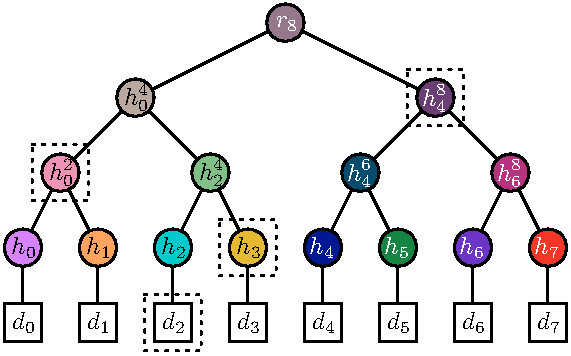
\includegraphics[width=\linewidth]{fig/mht-audit}
  \caption{Sample Merkle hash tree with eight leaf nodes. Dashed boxes indicate
  the nodes sent to prove the presence of the leaf $d_2$ in the tree.}
  \label{fig:mht-audit}
\end{figure}

A \emph{Merkle hash tree} is a binary tree in which each leaf node's value
represents data and each non-leaf node's value is the hash of its children's
values~\cite{merkle1988digital}. As shown in \autoref{fig:mht-audit}, the
structure of a Merkle hash tree allows one to efficiently prove that a data item
is present in the tree. Specifically, given the value of the root node of the
tree, one can verify the presence of any leaf node in the tree by computing a
number of hashes that is logarithmic in the number of data items in the tree.

A Merkle hash tree can store any number of nodes, i.e., the tree does not need
to be balanced. While several ways of computing the hashes in a non-balanced
tree exist, in this paper we use the method used in \ac{ct}~\cite{rfc6962}.
Specifically, given $n$ items in the Merkle hash tree, let \hashfunc be a hash
function, $d_i$ the $i$th data item (indexed from 0), and $a$ and $b$ integers
such that $0 < a < b \le n$. Then the hash of a non-leaf node representing the
$a$th to the $(b-1)$th data items is defined as
\begin{equation}
  \nodehash_a^b =
  \begin{cases}
    \hashfunc(0 \| d_a) & \mathrm{if\ } b = a + 1 \\
    \hashfunc(1 \| \nodehash_a^k \| \nodehash_k^b) & \mathrm{otherwise}
  \end{cases}
\end{equation}
where $\|$ denotes concatenation and $k = a + 2^{\lceil \log_2(b-a) \rceil - 1}$
(the largest power of 2 strictly less than $b - a$). For convenience, if $b = a
+ 1$ we write the hash as $\nodehash_a$ and call this a \emph{leaf hash}, and if
$a = 0$ and $b = n$ then we write the hash as $r_n$ and call this the \emph{root
hash}.

\begin{figure}
  \centering
  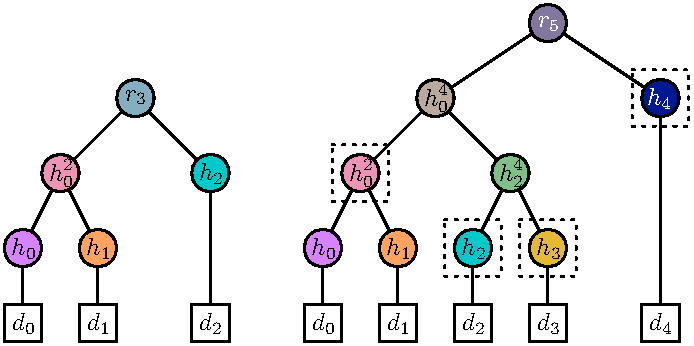
\includegraphics[width=\linewidth]{fig/mht-consistency}
  \caption{Sample Merkle hash trees with three and five data items,
  respectively. Dashed boxes indicate the nodes sent to prove consistency
between the root hashes $r_3$ and $r_5$.}
  \label{fig:mht-consistency}
\end{figure}

A Merkle hash tree can be used to implement an append-only, tamper-proof
log~\cite{crosby2009efficient}. As stated above, a Merkle hash tree can provide
an efficient \emph{proof of presence} for a given data item in the tree, thus
proving that an item was logged. To prove that the log is append-only, that is,
that no items have been changed or removed from the log, we can also use a
Merkle hash tree to provide an efficient \emph{proof of consistency} that is
logarithmic in the current size of the tree. As shown in
\autoref{fig:mht-consistency}, a proof of consistency allows one to compute the
root hash at two different times, thus showing that nodes have only been added
to the tree. A tamper-proof log would periodically sign and broadcast its root
hash, allowing clients to verify that it is not tampering with previously logged
data.

\subsection{Certificate Transparency}
\label{sec:background:ct}

\begin{figure}
  \centering
  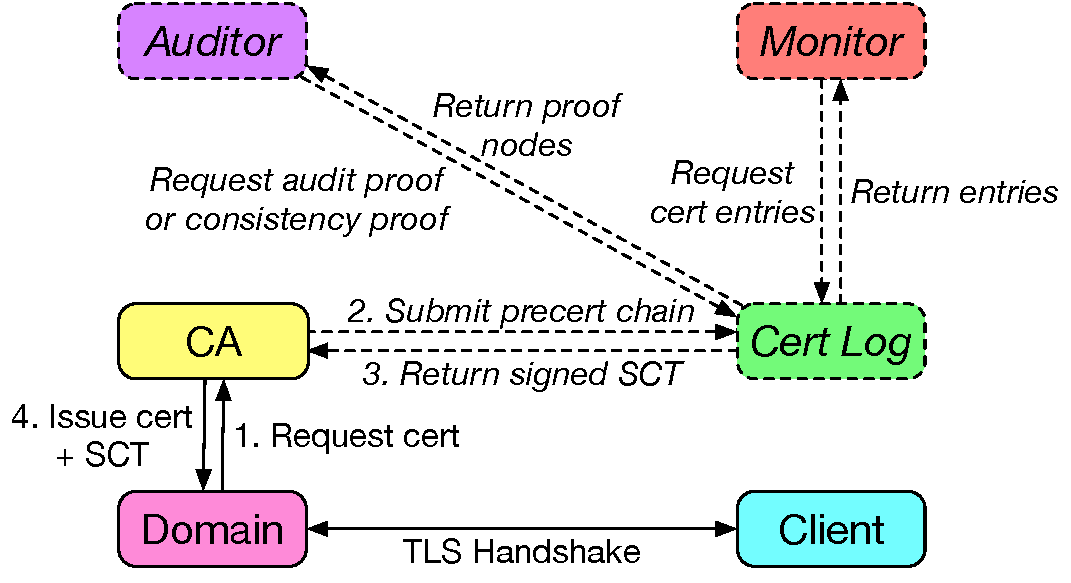
\includegraphics[width=\linewidth]{fig/ct}
  \caption{One possible configuration of the \ac{ct} architecture. Numbered
  steps denote the certificate issuance process. Dashed lines and boxes denote
entities or functions introduced by \ac{ct}, with their descriptions in
italics.}
  \label{fig:ct}
\end{figure}

\acf{ct} is a project by Google focused on enabling widespread detection of
certificate issuance~\cite{rfc6962}. As shown in \autoref{fig:ct}, \ac{ct}
introduces several new roles to the \ac{ca}-based ecosystem. \emph{Certificate
logs} are entities who record \ac{ca} behavior by maintaining a publicly
auditable, append-only, tamper-proof database of certificates. \emph{Monitors}
periodically retrieve these certificates to check for suspicious \ac{ca}
behavior, such as an obscure \ac{ca} issuing a certificate for Google.
\emph{Auditors} check for correct log behavior by periodically asking for
\emph{audit proofs}, which show that one or more certificates are in a log
database, or \emph{consistency proofs}, which show that the existing database
has not been tampered with, i.e., that no certificate has been changed, deleted,
or retroactively added to the log database.

A log leverages Merkle hash trees to implement its certificate database. As
explained above, the use of a Merkle hash tree allows a log to provide efficient
proofs of presence (i.e., audit proofs) and proofs of consistency (i.e.,
consistency proofs). While anyone may submit a certificate to a log, in current
practice \acp{ca} usually log certificates during the issuance process, as
depicted in \autoref{fig:ct}. Because attempting to update the Merkle hash tree
in real time may delay or block the certificate issuance process, logs define a
\emph{\ac{mmd}}, a time period after which a certificate is guaranteed to be
logged, and instead return a \emph{\ac{sct}}, which is effectively a promise to
add the certificate within the \ac{mmd}. The \ac{sct} is embedded into the
\ac{ca}-issued certificate as an X.509 extension and used to signal that a
domain uses \ac{ct} and that its certificate has been logged. Alternately, the
domain can send extra information such as \acp{sct} or audit proofs in the
\ac{tls} handshake using a \ac{tls} protocol extension.

%\draft{Monitoring and auditing details. Monitors periodically downloads all new
  %entries and verifies consistency proof. Does not need to keep cert entries
  %after finishing. Auditors periodically query for random audit proofs or
  %consistency proofs. Specifically, can pass a cert hash and a size of the tree
  %and get an audit proof in return, or pass two sizes of the tree and get a
  %consistency proof in return. To verify this information, log also provides a
  %function to get the latest signed tree head. In order to detect
  %\emph{equivocation} (i.e., showing different versions of the log to different
  %queries), auditors must gossip tree heads. The log's public key is known
  %through a trusted entity such as Google.}

%\draft{\ac{ct} does not check for revocation, though multiple extensions
%designed to handle revocation have been proposed (see \autoref{sec:related}).
%Perhaps the easiest way to do to this is to create a new Merkle hash tree every
%\ac{mmd} that contains as its leaves the list of \emph{currently valid}
%certificates.}

\subsection{Specifying and Inferring Domain Policy}
\label{sec:background:policy}

Previous work has proposed the use of domain-specified policies to protect
against \ac{mitm} attacks. In AKI~\cite{kim2013accountable} and its successor
ARPKI~\cite{basin2014arpki}, these policies are embedded within the certificates
themselves and specify attributes such as trusted \acp{ca} and public logs as
well as a ``cool-off period'' that forces potentially malicious certificates to
be visible in logs for some period of time before client can accept them. In
PoliCert~\cite{szalachowski2014policert}, the policies are stored separately in
logs. Other work, such as Blockstack~\cite{ali2016blockstack} or
IKP~\cite{matsumoto2017ikp}, has proposed placing policy information into a
blockchain. While IKP's policies operate similarly to those of PoliCert,
Blockstack simply provides the domain's keys directly. Of these proposals, only
ARPKI leverages the relationship between \acp{ca} and logs to ease the burden on
the domain during certificate issuance, but all proposals require the domain to
specify its policy in detail to prevent \ac{mitm} attacks resulting from
misbehaving \acp{ca}.

There has also been some work that takes a heuristic approach, using the past
behavior of \acp{ca} in order to determine how clients should trust them. For
example, CAge~\cite{kasten2013cage} propose a system that displays a browser
warning to users for certificates whose names are under a DNS top-level domain
that the issuing \ac{ca} has never signed for before. Perl, Fahl and Smith
propose to outright remove root certificates that have not been used to sign
(either directly or through \ac{ca} delegation) any observed certificates in the
past~\cite{perl2014you}. Both of these proposals use data from
Censys~\cite{durumeric2015search} or its predecessors, but do not use any
information from the domains themselves. Because of this, these approaches may
encounter situations where they mistake a legitimate, domain-initiated change
with an attempted \ac{mitm} attack and thus block a user from visiting a benign
site or expose a user to the \ac{mitm} attack. Indeed, a previous study of
changes in the Web \ac{pki}'s trust graph suggests that legitimate changes and
attacks share properties to the point that they cannot be easily
distinguished~\cite{amann2013no}.

\subsection{Signaling \ac{https} Deployment}
\label{sec:background:signaling}

Although \ac{hsts}~\cite{rfc6797} enforces the use of \ac{https} for a site
after a client has connected with that site over \ac{https} for the first time,
previous work has acknowledged the difficulty (in terms of both storage and
latency overhead) of identifying \ac{https}-deploying domains before the first
visit. The prevailing solution among browser vendors is \emph{\ac{hsts}
preloading}~\cite{keeler2012preloading}, in which browser vendors include a list
of the most popular sites that have deployed \ac{https}. These lists are
incomplete (covering only \steve{TODO: fill in} names in Chrome), and domains
must explicitly opt into adding themselves. As indicated by vendor-provided
guidelines,\footnote{\url{https://hstspreload.org/}} this process is prone to
mistakes by domain operators that lead to site inaccessibility.

As described in \steve{TODO: refer to previous section if mentioned elsewhere},
most approaches to disseminating certificate revocation information fail for
signaling because they rely on assumptions that do not hold in the signaling
problem. In particular, the use of \acp{crl}~\cite{rfc5280} does not scale to
the number of \ac{https}-deploying sites because we cannot assume that the
number of sites deploying \ac{https} will remain small compared to the overall
number of sites. More efficient versions of \acp{crl} also do not work: an
approach similar to Chrome's CRLsets~\cite{langley2012revocation} suffers from
the same incompleteness and opt-in hurdles mentioned above, and an approach
similar to CRLite~\cite{larisch2017crlite} relies on knowledge of all domain
names, which is infeasible in today's DNS due to many country code top-level
domains keeping their registries private. Approaches such as storing data in a
2-3 tree~\cite{naor1998certificate} or aoptimized Merkle hash
tree~\cite{laurie2012revocation}, while able to provide efficient proofs of
\ac{https} deployment, require online checks by clients, greatly increasing the
latency of connection establishment.

DANE~\cite{rfc6698}, which uses DNS to send a public key, certificate, or
\ac{ca} that the client should expect, can provide both signaling and policy
management with little added latency and without requiring browsers to store any
kind of signaling information. However, DANE relies on DNSSEC~\cite{rfc4033},
and both have a low deployment rate in today's
Internet,\footnote{\url{http://secspider.verisignlabs.com/stats.html}, retrieved
1 August 2017} with only 5,885 DANE records for \ac{https} and 1.67M verified
DNSSEC zones out of more than 329M names overall~\cite{dnib-14-1}. Changing
these numbers would require significant deployment efforts on the parts of
domains, including registering domain names through the subset of DNS registrars
that offer DNSSEC, usually as a paid service.


\section{Overview}
\label{sec:overview}

\begin{figure}
  \centering 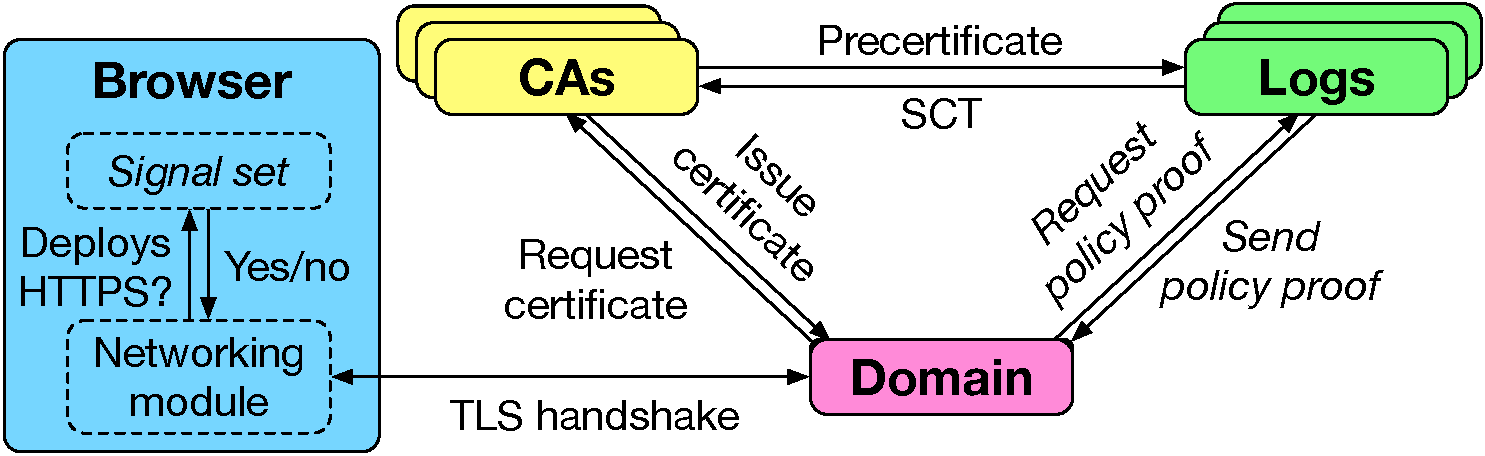
\includegraphics[width=\linewidth]{fig/overview} \caption{Overview
    of \ac{name} architecture (log auditors and monitors not shown). The browser
    is part of the client. Dotted lines denote browser components, and italic
    text denotes new components or actions in \ac{name}.}
  \label{fig:overview}
\end{figure}

In this section, we present a high-level overview of \ac{name}. We first present
one of our central insights and then describe the \ac{name} architecture. We
then provide an intuitive explanation for the policy and signaling mechanisms.

To move towards \iac{pki} with increased resilience to the compromise of trusted
parties (i.e., \acp{ca}), we need to prevent \iac{ca} that misissues a
certificate for a domain from exposing that domain to \iac{mitm} attack. We
observe that \steve{more signatures means more trust}, and therefore we design
\ac{name} around the idea that domains should be able to obtain and communicate
the presence of multiple signatures on a certificate. We can then protect
domains from \ac{mitm} attacks by simply communicating to the client the number
of signatures to expect. This approach results in simple policies that require
domain involvement only in rare cases of deliberate misissuance, and allow
security-conscious domains to ``ratchet up'' their security to their desired
level.

\ac{name} leverages \ac{ct}'s infrastructure in its policy mechanism, and
therefore the two systems have similar architectures, as shown in
\autoref{fig:overview}. \steve{TODO: add Censys data and an external service or
browser vendor to the overview figure} \ac{name} assumes a full deployment of
\ac{ct}, that is, all certificates must be logged for clients to accept them as
valid. Beginning in October 2017, Chrome will begin enforcing this requirement
for all \ac{https} sites, so this assumption is a reasonable one. For the
purposes of obtaining \acp{sct}, the logging process works just as it does in
\ac{ct}. Also as with \ac{ct}, public logs are kept accountable by auditors and
monitors, and an external party (Google in the case of \ac{ct}) maintains a list
of known trusted logs.

In \ac{name}, however, logs maintain an additional database of certificate
policies alongside their database of certificates. The logging process also
triggers changes in this policy database. Domains periodically request the proof
for their latest policy from the logs and provide both their policy and proof to
clients during the \ac{tls} handshake. We further describe the details of our
policy mechanism in \autoref{sec:policy}.

Client browsers locally maintain a \emph{signal set}, which indicate whether or
not a given domain has deployed \ac{https}. The networking module of the browser
(which handles the establishment of \ac{https} connections) queries the signal
set upon requesting a connection to a site in order to determine whether or not
to expect a certificate. If the signal set indicates that the domain has
deployed \ac{https} but the server does not provide a certificate, the browser
aborts the connection and displays an error message.

The signal set is created by using data from Censys~\cite{durumeric2015search},
which provides regular scans of the IPv4 address space on port 443, usually
reserved for \ac{https}. This data is used to construct a list of all DNS names
for which a \ac{tls} certificate has been observed (either as the main subject
or as a subject alternative name). This list is then represented using
\iac{dafsa} that recognizes the DNS names of sites that deploy \ac{https}. By
using compression techniques, we compact this \ac{dafsa} into a representation
that requires little storage. Such a compact representation allows us to store
the \ac{dafsa} in memory, offering performant lookups. We further describe the
details of our signal set design in \autoref{sec:signaling}.

%In particular, in \ac{name} we make use of a \emph{signal set},
%stored locally by client browsers. Browsers query for the presence or absence of
%a given domain name in the signal set to determine whether that domain has
%deployed \acs{https}. Because Censys~\cite{durumeric2015search} currently
%reports that close to 70 million known domains deploy \ac{https} and Verisign
%reports almost 330 million domain names overall~\cite{dnib-14-1}, we design our
%signal set to be scalable to hundreds of millions \steve{or billions, hopefully}
%of names, while taking up minimal space on client devices and supporting
%efficient membership queries. While \ac{ct} leverages public append-only logs to
%ensure that any \ac{ca} misbehavior for domains that have deployed \ac{https}
%must be made publicly visible before \iac{mitm} attack, the use of a signal set
%prevents an attack that can be made even with full \ac{ct} deployment, in which
%an adversary tries to fraudulently convince a client that a domain has not
%deployed \ac{https}. In \autoref{sec:signaling}, we provide a detailed
%look at our signal set design.

%\ac{name} further adds misbehavior prevention to the misbehavior detection
%capabilities of \ac{ct} through the use of \steve{policies for domains
  %maintained at public logs}. Specifically, public logs in \ac{name} maintain
  %policies for each domain that encode \steve{\acp{ca} authorized to issue
  %certificates for a domain or the number of independent certificate chains a
%domain must present to the client}. In contrast to other extensions of \ac{ct}
%that use log-based certificate policies such as
%PoliCert~\cite{szalachowski2014policert}, these policies do not need to be
%directly specified by the domain. \steve{I suppose this leaves out authorized
  %\ac{ca} specification unless we are willing to admit errors using a heuristic
%approach.} In \autoref{sec:policy}, we provide a detailed look at our policy
%mechanism.

%For comparison, we first present a
%purely DNS-based approach.

%\subsection{DNS-Based Policy}

%DANE~\cite{rfc6698} allows domains to specify policies (in the form of TLSA
%resource records in DNS) governing their public key certificates. Specifically,
%domains can specify
%\begin{compactenum}
%\item a CA certificate or public key that must appear in that domain's
  %certificate chain,
%\item a leaf certificate or public key that must be sent by the domain to the
  %client during the TLS handshake,
%\item a certificate or public key that must be used as the trust anchor of a
  %certificate chain (effectively allowing the domain to declare its own root
  %CA), or
%\item a leaf certificate or public key that must be sent by the domain to the
  %client, but does not need to be chained to a client-accepted root CA (i.e.,
  %the domain effectively sends a self-signed certificate).
%\end{compactenum}
%DANE thus provides domains with a great deal of flexibility: domains can prevent
%certificates issued by other misbehaving CAs or those certifying any other key
%from being accepted by clients, and domains can even eschew the CA hierarchy
%altogether by specifying their own trust roots or certificates.

%If a domain continues to obtain certificates from CAs, it can make use of the
%Certificate Authority Authorization (CAA) resource record~\cite{rfc6844}, which
%allows the domain to specify which CAs are authorized to issue certificates for
%the domain. In contrast to its counterpart in DANE, however, a CAA resource
%record is checked by CAs when the certificate is issued. Before issuing a
%certificate for a domain, a CA should check if a domain has a CAA resource
%record and ensure that the CA's name is present in the record. Though nothing
%stops a misbehaving CA from failing to check for a CAA resource record, the
%CA/Browser Forum has recently made this checking
%mandatory,\footnote{\url{https://cabforum.org/2017/03/08/ballot-187-make-caa-checking-mandatory/}}
%meaning that any CA that wants to continue issuing EV certificates (a capability
%granted by the CA/Browser Forum) must perform this check.

%With these systems in place, a domain can register its DNS name and obtain
%DNSSEC resource records (either creating these records itself if it manages its
%own nameserver or having its registrar manage the records). The domain can then
%create a CAA record restricting the CAs that can issue certificates for the
%domain (if obtaining CA-issued certificates), and also create a TLSA record to
%communicate this information to clients. Clients can then determine criteria for
%the domain's certificate chain upon receiving the DNS response, and use this
%information to determine whether or not to accept the presented certificate
%chain during the TLS handshake.

%A number of shortcomings exist with this approach. First, an adversary only
%needs to compromise a single private key (that of the registrar) to generate an
%unauthorized certificate that will be accepted by clients. Namely, the adversary
%can create a false TLSA record for a domain and use this to present a
%certificate (even a self-signed one) that the client would accept. However, the
%adversary cannot carry out targeted attacks this way (because DNSSEC must return
%a consistent response for all queries), and thus the attack can be detected
%(though not prevented). Moreover, this approach requires reliance on DNSSEC for
%security (deployed by a very small number of domains today).

%\subsection{Signaling Multiple Chains}

%A domain can signal that it has multiple certificate chains in one of two ways.
%The domain can signal the number of certificate chains the client should expect
%through DNS or register this number with browser vendors, who then periodically
%push a collection of these values to clients.

%To signal the number of expected certificates through DNS, the domain simply
%creates a special DNS record that indicates a value representing represents the
%minimum number of certificate chains the client should expect. Specifically, we
%allow the domain to create a DNS TXT record~\cite{rfc1035} containing a string
%of the form \texttt{domain-min-chains-N} where \texttt{N} is the number of
%certificate chains that the client should expect. Alternately, we propose a new
%DNS record called the TLSC record whose resource data consists of a single octet
%representing the number of chains.

%For security purposes, the domain should authenticate the above records with
%DNSSEC. However, the deployment rate of DNSSEC is currently quite low at around
%$0.6\%$ of the most popular sites~\cite{matsumoto2017ikp}. We thus expect that
%few domains will make use of this approach in practice; nevertheless, we allow
%this approach in addition to the one below to ensure that domains can easily
%signal the use of multiple certificate chains.

%To signal the number of expected certificates through the browser, the domain
%contacts one or more \emph{registration authorities}. At a high level, these
%registration authorities maintain an authenticated mapping of domain names to
%the minimum number of independent certificate chains that the client should
%expect. Because the set of domain names is finite (though large, at around 330M
%names in total) and the set of domains with multiple certificate chains is
%expected to be relatively small, we can leverage a set of filter cascades
%similar to that of CRLite~\cite{larisch2017crlite}. In particular, we can assume
%that the majority of domains will continue to use only a single certificate
%chain, with the number of domains using $n$ certificate chains falling sharply
%as $n$ increases. Let $U$ be the set of all domains, so $|U|$ is the number of
%all domains. Then, following the CRLite analysis, even in the absolute worst
%case (the number of domains with multiple certificate chains is $|U|/2$), a
%filter cascade would be about $0.35|U|$ bytes in size.

%\subsection{Multi-Chain Handshake}

%\begin{figure}
  %\centering
  %\begin{msc}{}
    %\setlength{\instdist}{6.0cm}
    %\setlength{\envinstdist}{1.0cm}
    %\setlength{\instwidth}{0.9cm}
    %\declinst{cli}{\scriptsize{Client}}{}
    %\declinst{dom}{\scriptsize{Domain}}{}

    %\mess{\scriptsize{ClientHello}}{cli}{dom}
    %\nextlevel
    %\mess{\scriptsize{ServerHello, Chains, ServerKeyExchange,
    %ServerHelloDone}}{dom}{cli}
    %\nextlevel
    %\mess{\scriptsize{ClientKeyExchange, ChangeCipherSpec, Finished}}{cli}{dom}
    %\nextlevel
    %\mess{\scriptsize{ChangeCipherSpec, Finished}}{dom}{cli}
  %\end{msc}
  %\caption{Message sequence diagram for the multi-certificate handshake. The
  %messages sent are identical to those for the \ac{tls} handshake except that
%multiple certificate chains can be sent in the handshake.}
  %\label{fig:handshake}
%\end{figure}

%In order for clients to process multiple certificate chains, we modify the
%standard \ac{tls} handshake as shown in \autoref{fig:handshake}. Our handshake
%differs from that of \ac{tls} only in the Chains message, which allows the
%server to send one or more certificate chains rather than a single chain.

%As in \ac{tls}, each chain must begin with the domain's certificate (i.e., the
%subject name of the certificate is the domain's DNS name), and in each chain,
%each certificate must be certified by the one following it. We add the
%requirement that the set of certificate chains must certify a common key.
%Ideally, the leaf certificate of each chain would specify the same key, but we
%do not assume that this will be possible for all domains.

%To allow domains to keep their existing \ac{tls} public keys while
%transitioning to a multi-chain ecosystem, we introduce an extension to
%\acs{x509} certificates called the \emph{Subject Alternative Key} extension.
%This extension allows a domain to specify additional key identifiers in
%\iacs{x509} certificate. Specifically, the extension consists of \iac{oid}
%assigned to the extension and a sequence of key identifiers encoded as octet
%strings. A key identifier is a unique value derived from a public key, such as
%the SHA-3 hash of the public key (other methods for generating key identifiers
%are discussed in RFC 5280~\cite{rfc5280}).

%The client then validates the set of certificate chains by verifying the
%following:
%\begin{compactitem}
%\item Each certificate
  %\begin{inparaenum}
  %\item has a valid signature,
  %\item is currently valid according to its NotBefore and NotAfter validity
    %period, and
  %\item has no critical \acs{x509} extensions that the client cannot process,
  %\end{inparaenum}
%\item With the exception of the last certificate in each chain, the signature on
  %each certificate can be verified with the public key listed in the Subject
  %Public Key field of the following certificate in the chain, or with the public
  %key of a root \acs{ca} known to the client.
%\item Each chain has a certificate that can be verified with the public key of a
  %root \ac{ca} known to the client.
%\item There exists a public key $K$ such that in each chain, the first
  %certificate of the chain contains $K$ as its Subject Public Key or as a
  %Subject Alternative Key.
%\end{compactitem}



\section{Signaling HTTPS Deployment}
\label{sec:signaling}

In this section, we describe the details of how we signal \ac{https} deployment
in \ac{name}.

\subsection{Data Sources}

The authors of CRLite~\cite{larisch2017crlite} observed that
Censys~\cite{durumeric2015search} and Google's set of \ac{ct}
logs\footnote{\url{https://www.certificate-transparency.org/known-logs}} have
played a critical role in making the set of all currently known \ac{tls}
certificates easily accessible. While the authors of CRLite used this knowledge
to space-efficiently store the set of all revoked certificates, in \ac{name} we
are interested in space-efficiently storing the set of all domains that have
deployed \ac{https}. We note that we can use the same data sources as CRLite
does and simply extract the set of domain names appearing in currently valid
certificates to obtain a list of all domains deploying \ac{https}.

To this end, Censys provides a scan of the entire IPv4 address space on port 443
(the default port number for \ac{https}) and the resulting \ac{tls} handshake
attempts.  \steve{(todo) We also downloaded a dump of XX \ac{ct} logs and
extracted domain names from the certificates stored at these logs.} After
extracting the data from the \steve{(update) May 18, 2017} scan results
\steve{(todo) and from the \ac{ct} log databasse}, we obtained a list of
\steve{(update) just over 69 million} domain names that take up a total of
\steve{(update) 147 MB}. This set excludes duplicate domain names as well as
common names \steve{(todo) explain in background} that are invalid DNS names.

\subsection{Approaches}

\steve{This subsection is in note form, and for now is just to summarize the
approaches I have tried.}

CRLite makes use of filter cascades (based on Bloom filters) to efficiently
store the set of all revoked certificates in around 10 MB. However, CRLite's
approach relies on having access to the set of all known certificates, which
Censys and the \ac{ct} logs can provide. While it is possible to access many of
the top-level domain zone files in DNS (including \texttt{.com}), many of the
registrars of country-specific top-level domains do not publicize their
information. Moreover, CRLite relies on the \steve{reasonable} assumption that
only a small minority of certificates will be revoked. By contrast, the rate of
\ac{https} deployment cannot be bounded by such assumptions, particular with the
advent of services such as Let's Encrypt, which has already increased the
\ac{https} deployment rate in its early stages \steve{(todo) wording}.

Constructing the signal set by simply compressing the set of \ac{https} domains
is also possible. As with most data compression algorithms, there is a clear
tradeoff between speed and compression ratio. For example, using lz4
\steve{(todo) cite} takes less than a second to compress and decompress, but
only obtains a compression ratio of 2.26 (for a compressed size of 65 MB). Using
bzip2, on the other hand, takes just over 10 seconds and has a ratio of 3.68 (40
MB compressed). Using xz took 64 seconds and produced a ratio of 4.45 (33 MB
compressed), and the best performer, zpaq (with the largest block size), took
4.5 minutes and produced a ratio of 5.88 (25 MB compressed). Unfortunately,
decompression with zpaq is slow, taking 7 minutes, and thus cannot be used to
support real-time signal set checking.

Succinct data structures provide a way for us to encode the signal set in a
space-efficient way while supporting efficient membership queries in the
succinctly encoded state. If we build a trie (also called a prefix tree) based
on the reversed domain names (capturing the highly repeated use of TLDs), we can
use the LOUDS (level order unary degree sequence) representation of the prefix
tree to efficiently encode the tree. In particular, we can represent the full
signal set in 73.3 MB. \steve{We also tried the use of minimal acyclic finite
  state automata (MAFSAs), which can represent the same information as a trie in
fewer states. However, this approach is quite slow for the number of domains we
want to represent, and there are fewer ways of efficiently encoding MAFSAs,
which in our case are effectively directed acyclic graphs with labeled edges.}

\subsection{Client Procedure}

\steve{How the client actually performs the lookup}


\section{Policy}
\label{sec:policy}

In this section, we provide a detailed description of policy and log operations
in \ac{name}. We begin with a brief overview of how logs in \ac{ct} work and
their shortcomings as they apply to \ac{name}. We then describe each of the main
operations of logs in \ac{name}: initial registration, updates, overwriting, and
proofs.

\subsection{CT Log Background}

Public logs in \ac{ct} are responsible for publicizing the certificates that
\acp{ca} issue. According to the \ac{ct} specification, logs offer the following
functionality:

\begin{compactitem}
\item \texttt{submit-entry}: submit a certificate or precertificate (described
  below) along with a certificate chain to the log for inclusion.
\item \texttt{get-sth}: retrieve a signed and timestamped copy of the
  latest root hash of the log's Merkle hash tree, called \iac{sth}.
\item \texttt{get-sth-consistency}: retrieve a consistency proof given two
  \acp{sth} of the log.
\item \texttt{get-proof-by-hash}: retrieve an inclusion proof for a given leaf
  hash and desired Merkle hash tree size (representing the state of a log at a
  given point).
\item \texttt{get-all-by-hash}: retrieve an inclusion proof, \ac{sth}, and
  consistency proof given a leaf hash and desired tree size.
\item \texttt{get-entries}: given a start and end index, retrieve a range of
  entries (including the certificate and their \acp{sct}) as well as the latest
  \ac{sth}.
\item \texttt{get-anchors}: retrieve a list of the trust anchors of the log
  (that is, the set of certificates that all submitted certificate chains must
  be rooted in).
\end{compactitem}

\ac{tls} clients only need \acp{sct} to deem a certificate valid in \ac{ct}, and
the number of \acp{sct} required depends on the lifetime duration of the
certificate \steve{cite CT log plan}. Therefore, for those clients not
performing monitoring or auditing functions, not even the \ac{sth} is
necessary. This is because \ac{ct} only cares about the fact that a potentially
unauthorized certificate was publicized \emph{at some point}, and as long as the
log is operating correctly (i.e., including the certificate in its Merkls hash
tree after issuing \iac{sct}), misbehavior \emph{should} be detected at some
point.

\subsection{Logs in \ac{name}}

Logs in \ac{name} maintain a mapping between domains and their policy
information, in addition to the information they maintain as \ac{ct} logs.

\subsection{Initial Policy Registration}

The initial policy registration can be performed when the log has no entry for
the given domain. A log performs the initial policy registration when its
receives a certificate whose subject name does not match any domain that the log
has in its mapping. In this case, the log simply creates a new policy entry for
that domain and associates the submitted certificate's public key with the
domain. The policy value is set to be the default value of 1 (indicating that
a client should expect only a single logged certificate chain from the domain).

Each new public key or certificate needs to be bound to a policy ID as well as
to the domain itself. It should be impossible to bind a new key to a policy ID
without the approval of the policy holder. Thus the domain will need to provide
some additional information regarding its authorization of the addition or
removal of any public key or certificate.

We therefore want the policy ID to be stable or at least linkable given an
addition or deletion operation. We also want the ID to be used to authenticate
a signature authorizing the addition or deletion of a key.

\subsection{Policy Updates}

\steve{Policies can be strengthened (i.e., not updated in terms of content but
in terms of independent chains) by simply specifying the same policy.}

\subsection{Policy Overwriting}

\subsection{Log Policy Proofs}

\steve{The irrelevance of log inclusion or consistency proofs to clients does
not hold in \ac{name}. This is because clients need to be convinced that a
policy was logged and that no policy overwrites or updates have taken place
since (i.e., the client sees the latest version of the policy). (Actually, if
the policy was logged and is not the latest, that could still prevent many
\acp{ca} from issuing unauthorized certificates if using the authorized \ac{ca}
approach. If we use the number of independent chains approach, we could include
a Bloom filter--like structure that makes it difficult for an adversary to get
away with fewer certificates even by forging them. How secure are Bloom filters
to collision attacks, anyway?)}

\subsection{Other Operations}


\section{Registration Authority}
\label{sec:ra}

\subsection{Policy}
\label{sec:ra:policy}

In a nutshell, a policy associates a domain with the public keys it uses during
the TLS handshake; a policy thus effectively pins a set of public keys to a
domain. Specifically, a policy binds a domain name to a set of \emph{policy
public keys}, an \emph{update threshold}, a \emph{registration proof}, and a set
of \emph{authentication public keys}. We describe each of these components
below.

The policy public keys and update threshold are used to authenticate updates to
the domain's policy. Specifically, to update its policy, a domain must provide a
threshold number of signatures on the new desired policy, and each of these
signatures must successfully verify with a distinct policy public key. Such an
update mechanism allows each domain to tune its policy's security to a desired
level: a lower update threshold means that an adversary needs to compromise
fewer policy private keys to maliciously update a domain's policy, while a
higher update threshold means that a domain must generate more signatures
(resulting in more computation) and send more information (resulting in higher
bandwidth cost) to update its policy.

The registration proof is used when the domain registers or recovers its policy.
A proof consists of one or more certificate chains that meet certain criteria
and a signature on the new desired policy. The RA maintains a list of root keys
in which each of these chains must be anchored. A proof also has an attribute
called \emph{strength}, which represents the number of keys that must be
compromised to forge all certificate chains. As we describe below, the strength
of a proof can be efficiently computed.

Finally, the authentication public keys are a set of whitelisted keys for
clients. In other words, a client will not accept a public key as belonging to a
domain if it does not appear in the domain's set of authentication public keys.
Whitelisting keys rather than certificates means that the domain does not have
to change its policy each time it obtains a new certificate. \steve{how often do
keys change between certificates from the same CA?}

%The use of domain-specified policies to provide authentication information is
%not new. DANE~\cite{rfc6698} allows domains to communicate similar policies via
%DNS records. However, DANE relies on DNSSEC (otherwise, the records containing
%these policies cannot be authenticated), and does not enable trust agility:
%clients must trust DNS to validate a DANE record.
%PoliCert~\cite{szalachowski2014policert} provides a slightly richer range of
%policies, but also lacks 

\subsection{Registration Proof Strength}
\label{sec:ra:proof}

The strength of a registration proof can be efficiently calculated. For the
purposes of computing strength, we represent a registration proof as a set of
chains $\{C_1, \ldots, C_n\}$. Each chain can be represented as a sequence of
keys $C_i = (K_i^1, \ldots, K_i^{\ell_i})$ where $K_i^1 \in R$ (assuming that
$R$ is the set of the root keys allowed by the RA) and $K_i^{\ell_i} = K_D$. We
then transform this set of chains into a graph as follows: the set of vertices
$V$ consists of a source node $S$ along with two nodes for each $K$ where $K \in
C_i$ for some $i$ such that $1 \le i \le n$. For a given $K$, we label these
nodes as $K$ and $K'$. The set of labeled edges $E$ is defined as follows: $(S,
K_i^1) \in E$ for all $i$ where $1 \le i \le n$, and all such edges are labeled
with $\infty$. In addition, for all $i$ such that $1 \le i \le n$ and all $j$
such that $1 \le j < \ell_i$, $(K_i^j, {K_i^j}') \in E$ and all such edges are
labeled with 1. Finally, for all $i$ such that $1 \le i \le n$ and all $j$ such
that $1 \le j < \ell_i$, $({K_i^j}', K_i^{j+1}) \in E$ and all such edges are
labeled with $\infty$.

We can then consider these edge labels as capacities in a minimum cut problem
with $S$ as the source and $K_D$ as the sink. The minimum cut will go through
some number of edges labeled with 1, and each of these edges represents a key
that needs to be compromised in order to disconnect all certificate chains. Thus
the minimum cut in this graph represents the minimum number of keys that must be
compromised in order to forge the entire set of certificate chains.

\subsection{RA Overview}
\label{sec:ra:overview}

The RA maintains a mapping of domain names to policies, as well as information
pertaining to domain policy registration. Specifically, the RA has a list of
accepted root public keys for registration proofs, as well as a mapping of
domain names to their most recent registration proofs.

The RA offers an API consisting of five methods, covering initial registration,
updates using policy keys, recovery using a stronger registration proof, lookup,
and enumeration of the RA database. We describe each below. \steve{Add
algorithmic descriptions}

The \texttt{register} method takes as input a domain name, a registration proof
consisting of a set of certificate chains and a signature on the desired policy,
and the desired policy itself. The domain name cannot already be present in the
RA's mapping. For each certificate chain, the RA checks that the leaf key can be
used to verify the signature on the desired policy, that each certificate has a
valid signature and has not expired, and that the chain is rooted in the RA's
set of root public keys. The RA then computes the strength of the proof and
associates the desired policy with the domain name. It also stores the
registration proof and strength, associated with the domain name.

The \texttt{update} method takes as input a domain name, the new desired policy,
and a set of signatures on the above information. The RA checks that each
signature can be verified with a distinct policy public key, and that the number
of signatures is at least the update threshold. If these checks pass, the RA
stores the new policy in its domain-policy mapping.

The \texttt{recover} method takes as input a domain name, a new desired policy,
and a registration proof. The domain name must be present in the RA's mapping.
The RA checks the registration proof in the same way as for initial
registration, but also checks that the proof is stronger than the current
strength of the domain's proof. If this check passes, the RA associates the new
policy with the domain name and updates the domain's registration proof
strength. We note that the new desired policy can be the same as the domain's
current policy, thus allowing a domain to ``strengthen'' its own registered
policy.

The \texttt{lookup} method takes as input a domain name and returns its policy,
registration proof, and proof strength. The domain name must be present in the
RA's mapping.

The \texttt{enumerate} methods takes no inputs and returns a list of all domain
names registered at the RA.


\section{Discussion}
\label{sec:discussion}


\section{Related Work}
\label{sec:related}


\section{Conclusion}
\label{sec:conclusion}

\steve{TODO}


\bibliographystyle{IEEEtranS}
\bibliography{bib}

\end{document}
